\documentclass[12pt]{article}
\usepackage[utf8]{inputenc}
\usepackage[T1]{fontenc}
\usepackage{amsmath}
\usepackage{amsfonts}
\usepackage{amssymb}
\usepackage[version=4]{mhchem}
\usepackage{stmaryrd}
\usepackage{graphicx}
\usepackage[export]{adjustbox}
\usepackage{venndiagram}
\graphicspath{ {imagenes} }

\usepackage{tikz}

\newtheorem{Def}{\quad Definición}
\newtheorem{Note}{\quad Nota}
\newtheorem{Ejem}{\quad Ejemplo}
\newtheorem{Prop}{\quad Propiedad}
\newtheorem{Theorem}{\quad Teorema}


\title{Probabilidad}
\author{REYNA LEON  APARICIO}
\date{Agosto 2023}

\begin{document}

\maketitle

\section{Introducción}

Uno de los primeros juegos de azar es los dados, por lo que en la antigüedad se ocupaba un cubilete para contenerlos, moverlos dentro y luego arrojarlos sobre una superficie plana, en el juego existen diversas jugadas que se realizaban con estos, por lo tanto el jugador desea crear un análisis aleatorio del posible resultado  del objeto para valorar su ganancia o pérdida, sin importar el número de intentos sin éxito el cálculo de sus predicciones son incalculables. Un popular apostador conocido como el caballero de Meré, planteo la posibilidad de ganar a Blaise Pascal,el cual al mismo tiempo consulta con Pierre de Fermat por lo cual empiezan a intercambiar cartas, aunque no se conoce todo lo que escribieron son muy importantes para los primeros fundamentos de la probabilidad. Meré creyó que había encontrado una falsedad en el juego, observando que el comportamiento de los dados era diferente cuando se utilizaba un dado que cuando se utilizaban dos dados. Pero su comparación era errónea entre la probabilidad de sacar un seis con un solo dado o de sacar un seis con dos dados. Para este caballero debería existir una relación proporcional entre el número de jugadas para conseguir el efecto deseado en uno y otro caso. 

\subsection{Introducción a la Teoría de conjuntos}

\begin{Def}
La teoría de conjuntos se ocupa para expresar la relación entre los miembros y los objetos analizando sus propiedades para comprender y comunicar conceptos matemáticos de manera más fácilmente, es decir que estudia los conjuntos, los cuales se representan con mayusculas y los objetos con minusculas. 
\end{Def}

\begin{Def}
Un conjunto es una colección de elementos definidos que llevan las ideas de elemento y pertenencia, esto quiere decir que un elemento $ \omega $ pertenece al conjunto. Es decir los conjuntos también son objetos y, por lo tanto, a menudo pueden relacionarse entre sí utilizando diferentes símbolos y notaciones.  Por lo que un conjunto A se dice que es subconjunto de B si y solo si todo elemento de A es también un elemento de B, (A $ \subset$ B).
\end{Def}

El problema radico en que el caballero no tuvo en cuenta que al lanzar un dado se tiene un espacio muestral $ \Omega = \{ 1, 2, 3, 4, 5,6 \}$ por lo que obtener un seis en un lanzamiento es: $ \frac{1}{6} $, por otra parte lanzar dos dados nos da como resultado  $6^2 = 36$, por  tanto obtener una pareja de seis es $\frac{1}{36}$.

\begin{Def} 
Un espacio muestral es el conjunto de todos los resultados posibles que se pueden dividir en grupos de un experimento, es decir se forma con todos los resultados que ya no es posible desglosar más y se denota con la letra. 
\\
\begin{tabular}{| c | c | c | c | c | c | c | }
\hline Primer dado & \multicolumn{6}{ |c| }{Segundo dado} \\ 
\hline
&1 & 2 & 3 & 4 & 5 & 6\\ \hline
1&(1,1)&(1,2)&(1,3)&(1,4)&(1,5)&(1,6)\\ \hline
2&(2,1)&(2,2)&(2,3)&(2,4)&(2,5)&(2,6)\\ \hline
3&(3,1)&(3,2)&(3,3)&(3,4)&(3,5)&(3,6)\\ \hline
4&(4,1)&(4,2)&(4,3)&(4,4)&(4,5)&(4,6)\\ \hline
5&(5,1)&(5,2)&(5,3)&(5,4)&(5,5)&(5,6)\\ \hline
6&(6,1)&(6,2)&(6,3)&(6,4)&(6,5)&(6,6)\\ \hline
\end{tabular}

\end{Def}


\begin{Def} 
Un vento es un subconjunto del espacio muestral. 
\\
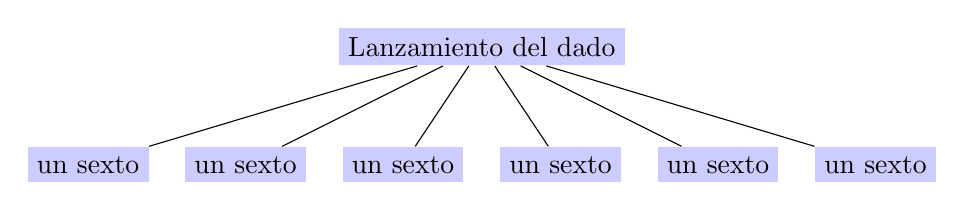
\begin{tikzpicture}[every node/.style={rectangle, fill=blue!20!white} ]
\node {Lanzamiento del dado} [sibling distance=2cm]
child {node {un sexto} 
}
child {node {un sexto} 
}
child {node {un sexto} 
}
child {node {un sexto} 
}
child {node {un sexto} 
}
child {node {un sexto} 
};
\end{tikzpicture}

\end{Def}


Otra manera mas clara de verlo seria considerando los siguientes eventos: 
\\
A: obtener un seis en el primer lanzamiento 
\\
B: obtener un seis en el segundo lanzamiento 

Entonces la unión de estos eventos se representan  en el siguiente diagrama: 


%\begin{figure}
\centering
\begin{tikzpicture}[set/.style = {draw,circle,minimum size = 0.7cm},scale=0.5]
%\draw (coordenada en x inf izq, coord en y supe izq) rectangle (coord x inf derecha,coord y sup der);
\draw (-12,12) rectangle (12,-12);
\node (A) at (-4.5,3.5)  [set] { \Large{(6,1),(6,2),(6,3),(6,4),(6,5)}};
\node (C) at (3.5,-4.5) [set] {\Large  {(1,6),(2,6),(3,6),(4,6),(5,6)}};
\node at (barycentric cs:A=1,C=1) [] {$(6,6)$};
\node at (3,-7.5) {\LARGE\textbf{B}};
\node at (-3,7.5) {\LARGE\textbf{A}};

\end{tikzpicture}
%\caption{La union de los eventos A y B} \label{fig:Regiones}
%\end{figure}



Además, dentro de los resultados posibles del experimento hay 24 resultados en los que no se obtiene un seis. Otra manera de verlo mas simple es: 


%\begin{figure}
\centering
\begin{venndiagram2sets}[labelOnlyA=5,labelOnlyB=5,labelAB=1, labelNotAB=24]
\end{venndiagram2sets} 
%\end{figure}


Por esta razón la probabilidad de obtener un seis en el primer lanzamiento o un seis en el segundo lanzamiento es igual a: 

$P(A \cup B)=P(A)+P(B)-P(A \cap B) = \frac{6}{36} + \frac{6}{36} - \frac{1}{36} = \frac{11}{36}$

Recordemos que el Caballero de Mere planteo que  

$P(A \cup B)=P(A)+P(B) = \frac{1}{6} + \frac{1}{6} = \frac{12}{36} = \frac{1}{3}$

por lo que $\frac{12}{36} \neq  \frac{11}{36}$ de este modo vemos que la proporcionalidad es falsa, ya que si dos eventos A y B son directamente proporcionales entonces $P(A) = kP(B)$, donde k es la constante de proporcionalidad 



\begin{Def} 
La probabilidad frecuentista refiere a experimentos que se pueden repetir indefinidamente con las mismas condiciones, por lo que los sucesos tienden a estabilizarse alrededor de un número fijo. Entonces debido a que para tener un doble seis al lanzar dos dados es $\frac{1}{36}$,para poder conseguir un 6 en uno de 37 lanzamientos de dos dados seria $37* \frac{1}{36} = \frac{37}{36} > 1$ .
\end{Def}


\begin{Def} 
Las operaciones entre conjuntos son los eventos que sepueden combinar para dar lugar a nuevos eventos. Por ejemplo si A y B son dos eventos entonces: \\
A $\cup$ B= \{(6,1),(6,2),(6,3),(6,4),(6,5),(6,6),(1,6),(2,6),(3,6),(4,6),(5,6),(6,6)\} \\
A $\cap$ B = \{ (6,6) \} \\
A - B = A $\backslash$ B = \{(6,1),(6,2),(6,3),(6,4),(6,5) \} \\
$A^c$ = \{(1,6),(2,6),(3,6),(4,6),(5,6) \}
\end{Def}





\begin{Def} 
La sigma-algebra es una clase de subconjuntos del espacio muestral sobre la que puede establecerse una probabilidad con una estructura mínima, ya que no puede ser una colección cualquiera de sucesos por lo que cumple:

$ \Omega \in A$ \\
Si $A \in A \rightarrow A^c \in A$ \\
Si $A_{1}, A_{2},... \in A \rightarrow A_{1} \cup A_{2} \cup ... \rightarrow \bigcup_{i=1}^{ \infty} A_{i} \in A $
\end{Def}


\begin{itemize}

\item Definición de Probabilidad

\end{itemize}


\section{ incluir}

\end{document}

